\documentclass{article}

\usepackage{amsmath}
\usepackage[margin=1in]{geometry}
\usepackage{listings}
\usepackage{hyperref}
\usepackage{graphicx}
\usepackage{amssymb}
\usepackage{verbatim}
\usepackage{siunitx}
\usepackage{enumitem}
\usepackage{bbm}
\usepackage{bm}
\usepackage{caption}
\usepackage{algpseudocode}
\usepackage{algorithm}
\usepackage[square,sort,comma,numbers]{natbib}

\newcommand{\norm}[1]{\left\lVert#1\right\rVert}
\newcommand{\normtwo}[1]{\left\lVert#1\right\rVert_2}
\newcommand{\abs}[1]{\left\lvert#1\right\rvert}
\newcommand{\mat}[1]{\bm{{#1}}}
\renewcommand{\vec}[1]{\bm{{#1}}}
\newcommand{\lequiv}{\Leftrightarrow}
\newcommand{\bigO}[1]{\mathcal{O}\!\left(#1\right)}
\newcommand{\ceil}[1]{\left\lceil #1 \right\rceil}
\newcommand{\floor}[1]{\left\lfloor #1 \right\rfloor}
\newcommand{\sfrac}[2]{#1/#2}
\newcommand{\hquad}{\enskip}
\newcommand{\expected}[1]{\mathbb{E}\left[#1\right]}
\newcommand{\mspan}[1]{\text{span}\left( #1 \right)}
\newcommand{\prob}[1]{P\left(#1\right)}
\newcommand{\probt}[1]{P\left( \text{#1} \right)}
\newcommand{\condprob}[2]{P\left(#1 \:|\: #2\right)}
\newcommand{\condprobt}[2]{P\left(\text{#1} \:|\: \text{#2}\right)}
\newcommand{\bayes}[2]{\frac{\condprob{#2}{#1}\prob{#1}}{\prob{#2}}}
\newcommand{\bayesx}[3]{\frac{\condprob{#2}{#1}\prob{#1}}{\condprob{#2}{#1}\prob{#1} + \condprob{#2}{#3}\prob{#3}}}
\newcommand{\sech}{\text{sech}}
\newcommand*{\qed}{\hfill\ensuremath{\blacksquare}}%
\newcommand*{\vertbar}{\rule[-1ex]{0.5pt}{2.5ex}}
\newcommand*{\horzbar}{\rule[.5ex]{2.5ex}{0.5pt}}
\newcommand{\vect}[2]{\underline{{#1}}_{{#2}}}
\newcommand{\basisp}[1]{\underline{{p}}_{{#1}}}
\newcommand{\basisq}[1]{\underline{{q}}_{{#1}}}
\newcommand{\coeff}[1]{\underline{{a}}_{{#1}}}
\newcommand{\bestfit}{\underline{\bar{x}}}
\newcommand{\grad}{\nabla}
\newcommand{\laplace}{\Delta}


\begin{document}
\section{Background}
The problem being solved is the Poisson problem in one dimension with variable coefficients:
$$ -\grad \cdot \left(k\left(\vec{x}\right)\grad\vec{u}\right) = f $$
$$ f(\vec{x}) = \vec{x} $$
Where $k\left(\vec{x}\right)$ is some function $k\: : \: \mathbb{R} \to \mathbb{R}$.  For constant $k$ this is equivalent to:
$$ -k\grad^2\vec{u} = f $$
The choice of $f\left(\vec{x}\right)$ is arbitrary and was chosen to produce interesting solution plots, but any $f\left(\vec{x}\right)$ should show similar convergence properties.  This differential equation is defined on the following domain with Dirichlet boundary conditions:
$$ \Omega = \left[-1, 1\right]$$
$$ \partial\Omega = 0 $$
This is discretized using second-order centered finite differences on a grid of $N=31$ equispaced points and results in the following system:
$$ \mat{A}\vec{u} = \vec{x} $$
where the $i$'th entry of $\mat{Au}$, $\left(\mat{Au}\right)_i$ is given by:
$$\left(\mat{Au}\right)_i = \frac{1}{h^2} \left( -k_{i-\frac{1}{2}} u_{i-1} + \left(k_{i-\frac{1}{2}} + k_{i+\frac{1}{2}}\right)u_i - k_{i+\frac{1}{2}}u_{i+1} \right)$$
$$h = \frac{1}{N+1}$$

Note that $k\left(x\right)$ is discretized on the \textit{midpoints} of the grid nodes instead of at the gridpoints.  This preserves the SPD structure of the system.

The above linear system is solved using a two-level V cycle multigrid method using the following steps:

\begin{enumerate}
\item Generate an initial guess of $0$, $\vec{u}_0 = \vec{0}$.
\item Pre-smooth the guess using one iteration of Jacobi using weight $\omega$.
\item Restrict the grid and residual using the operator $\mat{R}=\mat{P}^T$.  The given interpolation operator $\mat{P}$ is constructed as the \textit{ideal interpolation operator}, $\mat{P}=-\mat{A}_{ff}^{-1}\mat{A}_{fc}$.
\item Perform a direct linear solve on the restricted residual to obtain the coarse solution.
\item Interpolate the solution to the fine grid using operator $\mat{P}$.
\item Post-smooth using one iteration of Jacobi, with same weight $\omega$.
\end{enumerate}

The Jacobi smoothing weight that is used, $\omega$, is the optimal weight that minimizes the overall factor of convergence for the method:

$$\omega = \arg \min_{\omega\in\left(0,1\right)} \lim_{k\to\infty} \frac{ \vec{u}_{k+1} - \vec{u}^* }{ \vec{u}_{k} - \vec{u}^* }$$

where $\vec{u}^*$ is the ``optimal'' solution, precomputed by a dense linear solve.  Computationally, $\omega$ is approximated with a bracketed numerical optimization method, with the assumption that $\omega$ is unimodal with respect to the convergence factor.  If $\omega$ is not unimodal, which could possibly be the case for more complicated differential equations, then a more sophisticated method would be required to find the global optimum.

\section{Generating Coarse Grids}

To train the model, a set of grids of two types were generated via random perturbation.  These were generated for different problems, and their types are:
\begin{itemize}
\item poisson problem with a constant coefficient of 1 ($\laplace u = f$)
\item variable coefficient problems ($\grad \cdot \left(k\left(x\right)\grad u\right) = f$)
\end{itemize}

\subsection{Poisson with unitary constant coefficient}

For the constant-coefficient poisson problem, 96000 C/F grids were generated via random perturbation.  Several ``reference'' grids were generated according to varying coarsening factors, of which the following values were used:

$$r = \left\{
\frac{1}{9},\quad
\frac{1}{8},\quad
\frac{1}{7},\quad
\frac{1}{6},\quad
\frac{1}{5},\quad
\frac{1}{4},\quad
\frac{1}{3},\quad
\frac{1}{2},\quad
2,\quad
3,\quad
4,\quad
5,\quad
6,\quad
7,\quad
8,\quad
9
\right\}$$

where values of $r<1$ refer to grids where every $\frac{1}{r}$ points is a fine point and the rest coarse, and $r>1$ refers to grids with every $r$ points being a coarse point and the rest fine.  These grids were then used to solve the Poisson problem and their weights and convergence factors recorded.

Each reference grid was randomly permuted such that each grid point had a random probability of being flipped to the opposite value.  I.e. coarse point to fine, and fine point to coarse.  Random trials of the following probabilities were used:

$$ p = \left\{0.01, \quad 0.05, \quad 0.1, \quad 0.25, \quad 0.5, \quad 0.75\right\} $$

For each value of $p$, $1000$ random grids were generated according to the above permutation strategy.  Each random grid was then also used to solve the defined Poisson problem, and the optimal Jacobi weight, $\omega$, and convergence factor were recorded.

For this case, 16 convergence factors $\times$ 6 probability trials $\times$ 1000 random iterations = 96000 random grids were created.

\subsection{Variable-Coefficient Poisson}

The process of generating the variable coefficient grids is very similar to the constant case.  Again, several ``reference'' grids were generated according to different coarsening factors:

$$r = \left\{
2,\quad
3,\quad
4,\quad
5,\quad
6,\quad
7,\quad
8,\quad
9
\right\}$$

For the sake of time, only integer values of $r$ were used to create the grids.  Using the same $p$ values as above, $5000$ random grids were permuted for each value of $p$.  For each grid, a random function for $k$ is selected from the set:

$$
k\left(x\right) = \begin{cases}
\alpha & 0 < \alpha < 10 \\
\text{rand()}\left(\alpha + 1\right) & 0 < \alpha < 10 \\
\alpha\cos\left(\pi x \beta\right) + \gamma & 0 < \alpha < 10, 0 < \beta < 10, 0 < \gamma < 10\\
\left(\sum_{i=1}^5 \alpha_i x^i\right) + 0.01 & -10 < \alpha < 10 \end{cases}
$$

where the various coefficient values are randomly chosen so that the function of $k\left(x\right)$ is strictly positive.  A total of $240,000$ of these variable coefficient grids were generated, which equates to a total grid count of $336,000$.  The code used to generate these grids is given in \texttt{grids/gen\_grids.py}, and with slight modification can produce the unitary coefficient poisson grids as well.

\section{CNN Model}

In an attempt to predict both optimal Jacobi weight and factor of convergence given an arbitrary grid, a CNN of the architecture described below was trained.  The layers of this network were inspired by those used in Residual neural networks (ResNet) in which the output of a layer may ``skip'' over certain layers, thus speeding up training and allowing for deeper networks.  %A graphical description is given in Figure \ref{fig:architecture} and also an overview is described below:
An overview is described below:

%% \begin{figure}[t]
%%   \centering
%%   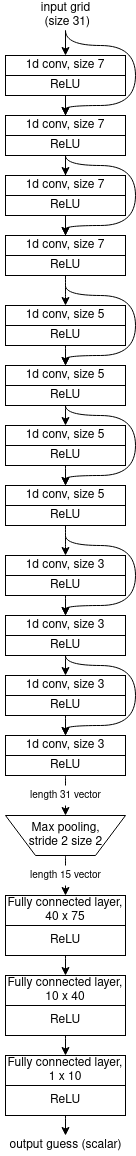
\includegraphics[scale=0.5]{figures/jacobi-conv/cnn_architecture.png}
%%   \caption{Architecture of the CNN with ``skipping'' akin to a ResNet.  These skips may avoid vanishing gradients and can simplify training of the network.}
%%   \label{fig:architecture}
%% \end{figure}

\begin{enumerate}
\item 6 1-dimensional convolution layers with kernel size 7.  Zero padding of size two is applied to the left and right to keep the output element the same shape --- this is for the residual architecture so that output vectors have equal dimensionality.  Each convolutional layer has a ReLU activation function.  The first layer takes two input layers and emits 10 output layers, subsequent convolutions have 10 input and output layers.  Even numbered convolution layers $k$ take as input both the output of layers $k-1$ and $k-2$, while odd numbered layers only take the output from layer $k-1$.
\item 6 1-dimensional convolution layers with kernel size 5.  Zero padding is applied.  ReLU activation.  10 input, 10 output layers.  Similar residual pushing strategy from above.
\item 6 1-dimensional convolution layers with kernel size 3.  Zero padding is applied.  ReLU activation.  10 input, 10 output layers.  Similar residual pushing strategy from above.
\item Max pooling layer with kernel size 2 and stride 2.
\item The tensor is flattened from dimensions $N \times 10 \times 15$ to $N \times 1 \times 150$.
\item Fully connected layer with input size 150, output size 132.  ReLU activation function.
\item Fully connected layer with input size 132, output size 113.  ReLU activation function.
\item Fully connected layer with input size 113, output size 95.  ReLU activation function.
\item Fully connected layer with input size 95, output size 76.  ReLU activation function.
\item Fully connected layer with input size 76, output size 57.  ReLU activation function.
\item Fully connected layer with input size 57, output size 39.  ReLU activation function.
\item Fully connected layer with input size 39, output size 20.  ReLU activation function.
\item Fully connected layer with input size 20, output size 1.  ReLU activation function.
\end{enumerate}

\subsection{Training}

The previously generated set of $240,000$ random grids was split into training and testing sets, with a random $85\%$ of entries going to the training set and the remaining $15\%$ going into the testing set.

The grids were formed into a $N\times 2 \times n$ tensor, with $N$ being the number of grids and $n=31$ being the grid size.  The dimension of $2$ in the second index allows the CNN to receive both the \textit{grid} and the \textit{coefficient values} as input.  The tensor representation was formed by means of assigning $1$ to coarse points and $-1$ to fine points:

\begin{align*}
T_{i1j} &= \begin{cases}
1 & \text{point $j$ in grid $i$ is coarse}\\
-1 & \text{point $j$ in grid $i$ is fine}
\end{cases}\\
T_{i2j} &= k\left(\frac{j}{n}\right)
\end{align*}

Where $k\left(x\right)$ is the coefficient function.  Note that even though this is discretized on the midpoints when the system is created, the CNN still receives the values of the function evaluated on the grid points.  This is to ensure that the input grid and the coefficients have the same shape.

The input weights and convergence factors were then normalized such that their range lies between $\left[0, 1\right]$.  When displaying any output from the CNN, this transformation must be undone for the results to be sensible.  The grid dataset class contains a \texttt{scale\_output()} method to do this in \texttt{jacobi-cnn/model.py}.

The CNN was separately trained for 20 and 30 epochs for the Jacobi weights and convergence factor models, respectively.  Training was done using a MSE (mean-square error) loss function with the \textit{Adam} optimizer.  In each iteration, minibatches of size $500$ were used to train and backpropagate the model.  Nothing special was performed for minibatch sizes under $500$, in the case that the total number of grids was not divisible by $500$.  The MSE loss and L1 loss at each iteration is given by Figures \ref{fig:jacobi_loss}, \ref{fig:conv_loss}.  These are also compared against the loss of a ``trivial predictor'', where the predicted value is simply the average of all input values.

\subsection{Results}

Results of plotting the true vs predicted Jacobi weights and convergence factors can be seen in Figures \ref{fig:jacobi_preds} and \ref{fig:conv_preds}, respectively.  Final MSE/L1 loss values are given in Table \ref{tab:loss}.

\begin{table}[t]
\centering
\begin{tabular}{|l|l|l|l|}
\hline
Model & Metric & Dataset & Value \\

\hline
Jacobi Weight & MSE & Training & 0.0018331280443817377 \\
Jacobi Weight & MSE & Testing & 0.0018395978258922696 \\
Jacobi Weight & L1 & Training & 0.029253767424938727 \\
Jacobi Weight & L1 & Testing & 0.029271099756634424 \\
\hline
Convergence Factor & MSE & Training & 0.001483894418925047 \\
Convergence Factor & MSE & Testing & 0.0015170895494520664 \\
Convergence Factor & L1 & Training & 0.023908496504070377 \\
Convergence Factor & L1 & Testing & 0.023865242609902033 \\
\hline
\end{tabular}
\caption{Final training MSE/L1 loss values for the two models.  Lower values correspond to higher model accuracy.}
\label{tab:loss}
\end{table}

\section{Discrete Grid Optimization}

In an attempt to find the most ``convergent'' grid, an implementation of the \textit{simulated annealing} optimizer was used to obtain the grid that minimizes both the convergence rate and C/F ratio (number of points on the coarsest level divided by the total number of grid points).  To minimize both metrics, each iteration of the simulated annealing algorithm alternates between optimizing either the convergence rate or the C/F ratio.  Thus, each pass steps either towards a more optimal C/F ratio, or more optimal convergence rate.  An overview is given in Algorithm \ref{anneal}.  The algorithm itself and helper methods are adapted from those in \citep{Bertsimas1993}.

As a sanity check, the optimizer was first run on \textit{only} the convergence factor (Fig \ref{fig:optimized_grid_poisson_conv}) and the C/F ratio (Fig \ref{fig:optimized_grid_poisson_cf}).  An example of optimizing both can be seen in Figure \ref{fig:optimized_grid_poisson}, though the final output is wildly dependent on the random input guess.  More tweaking to the parameters and the algorithm itself is likely needed.

\begin{algorithm}
  \caption{Simulated annealing}
  \label{anneal}
  \begin{algorithmic}
    \Function{anneal}{}
      \State $\mat{G} \gets $ generate\_random\_grid() \Comment{Generate random grid and evaluate obj. function}
      \State $\vec{\phi}_G \gets \phi\left(\mat{G}\right)$
      \For {$k \gets 1\ldots k_{\text{max}}$}
        \State $t := T\left(k/k_{\text{max}}\right)$ \Comment{Compute current temperature value}
        \State $\mat{S} := $ random\_perturb($\mat{G}$) \Comment{Generate a random next step, and evaluate obj. function}
        \State $\vec{\phi}_S := \phi\left(\mat{S}\right)$
        \State $i := k \mod\ 2$ \Comment{Alternate minimizing each metric}
        \If{$P\left(\vec{\phi}_G, \vec{\phi}_S, t, i\right) \geq $ random(0,1)}
          \State $\mat{G} \gets \mat{S}$ \Comment{Randomly take the next step according to the temperature}
          \State $\vec{\phi}_G \gets \vec{\phi}_S$
        \EndIf
      \EndFor
    \EndFunction
    ~\newline
    \Function{$\phi$}{$\mat{G}$} \Comment{Objective function to minimize}
      \State $c := $ CNN\_conv$\left(\mat{G}\right)$
      \State $w := \abs{\text{C points in }\mat{G}} / \abs{\text{total points in } \mat{G}}$
      \State \Return $\begin{bmatrix} c & w \end{bmatrix}^T$
    \EndFunction
    ~\newline
    \Function{T}{$r$} \Comment{Computes temperature of current iteration}
      \State
      \Return $\frac{1}{10\log\left(r\right)}$
    \EndFunction
    ~\newline
    \Function{P}{$e, e^\prime, T, i$} \Comment{Computes probability of switching grids}
      \State
      \Return $\exp\left(\sfrac{-\left(\vec{e}^\prime_i - \vec{e}_i\right)}{T}\right)$
    \EndFunction
\end{algorithmic}
\end{algorithm}


\begin{figure}[h]
  \centering
  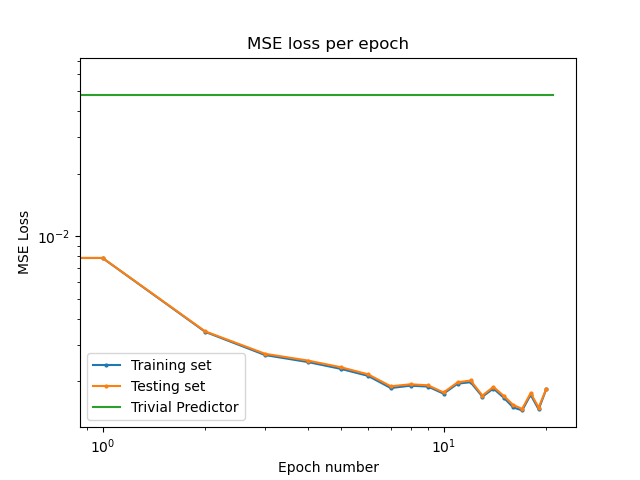
\includegraphics[scale=0.7]{figures/jacobi-conv/jacobi_mse.png}
  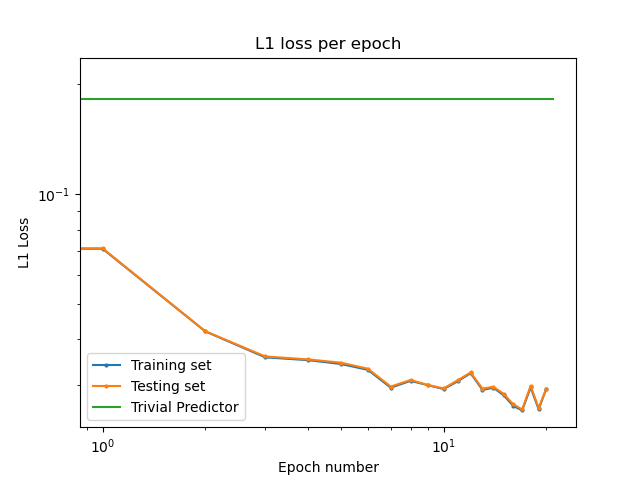
\includegraphics[scale=0.7]{figures/jacobi-conv/jacobi_l1.png}
  \caption{MSE, L1 loss per training iteration for Jacobi weights}
  \label{fig:jacobi_loss}
\end{figure}

\begin{figure}[h]
  \centering
  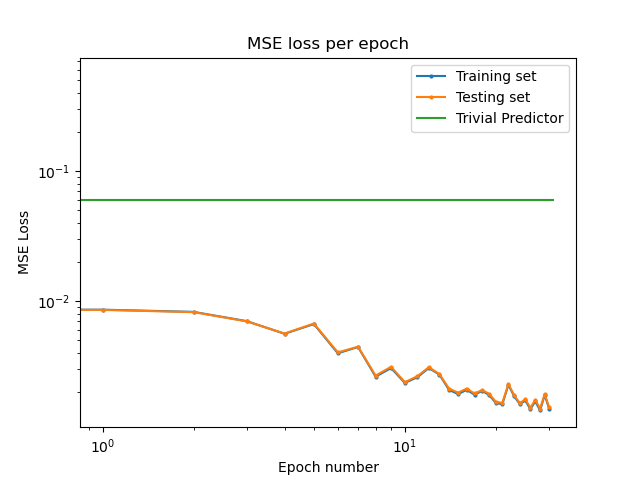
\includegraphics[scale=0.7]{figures/jacobi-conv/conv_mse.png}
  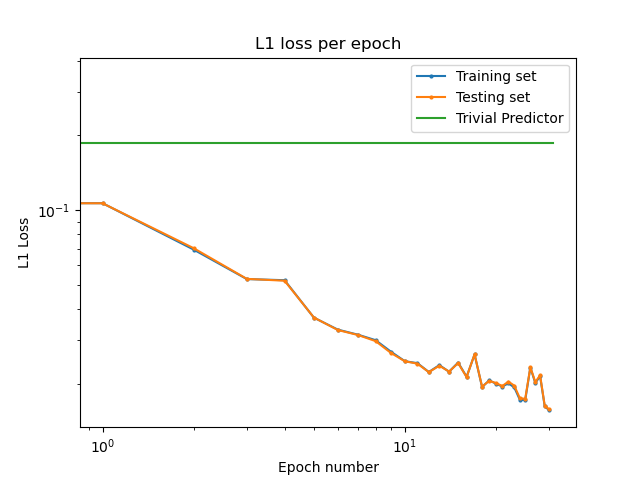
\includegraphics[scale=0.7]{figures/jacobi-conv/conv_l1.png}
  \caption{MSE, L1 loss per training iteration for convergence factor}
  \label{fig:conv_loss}
\end{figure}

\begin{figure}[h]
  \centering
  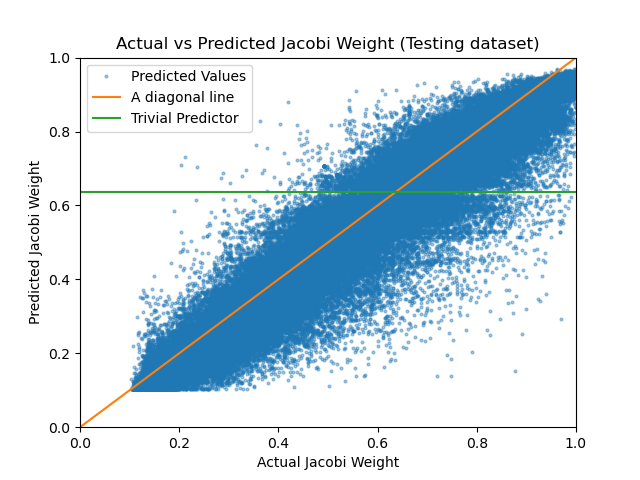
\includegraphics[scale=0.7]{figures/jacobi-conv/jacobi_test_pred.png}
  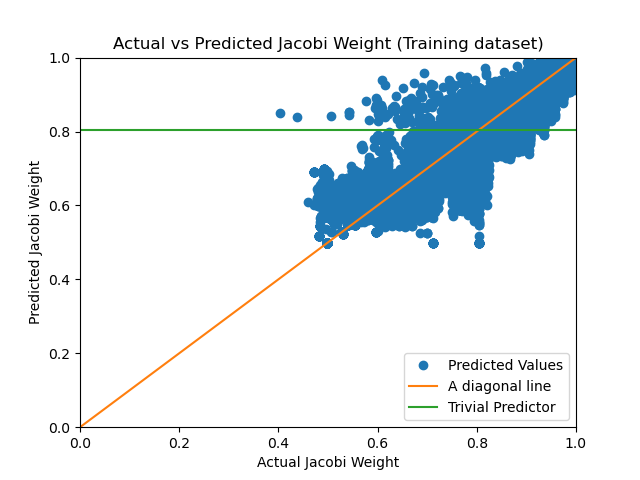
\includegraphics[scale=0.7]{figures/jacobi-conv/jacobi_train_pred.png}
  \caption{Predicted vs Actual Jacobi Weights}
  \label{fig:jacobi_preds}
\end{figure}

\begin{figure}[h]
  \centering
  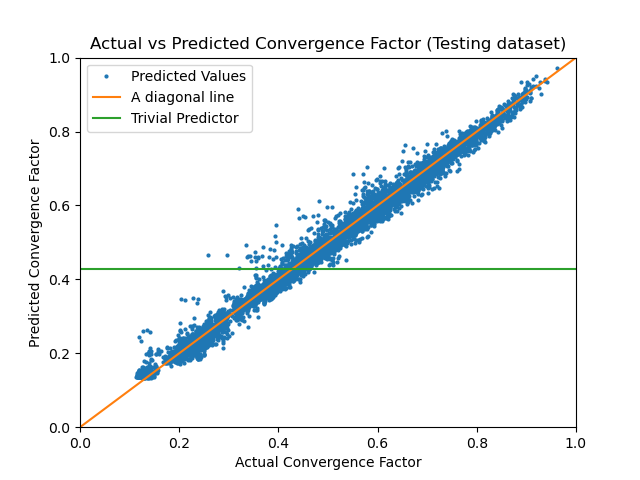
\includegraphics[scale=0.7]{figures/jacobi-conv/conv_test_pred.png}
  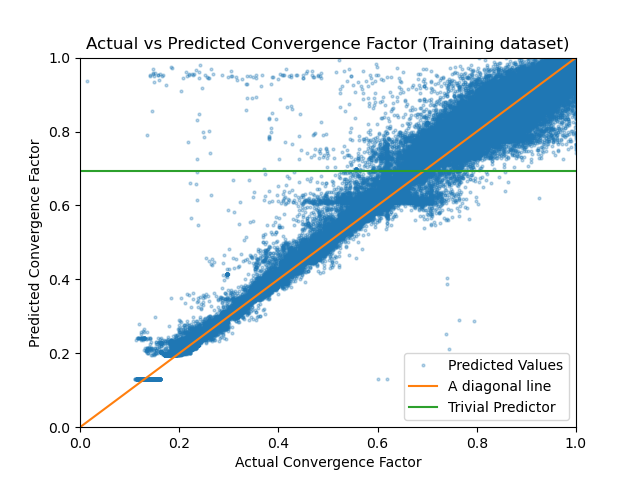
\includegraphics[scale=0.7]{figures/jacobi-conv/conv_train_pred.png}
  \caption{Predicted vs Actual Convergence Factors}
  \label{fig:conv_preds}
\end{figure}

\begin{figure}[h]
  \centering
  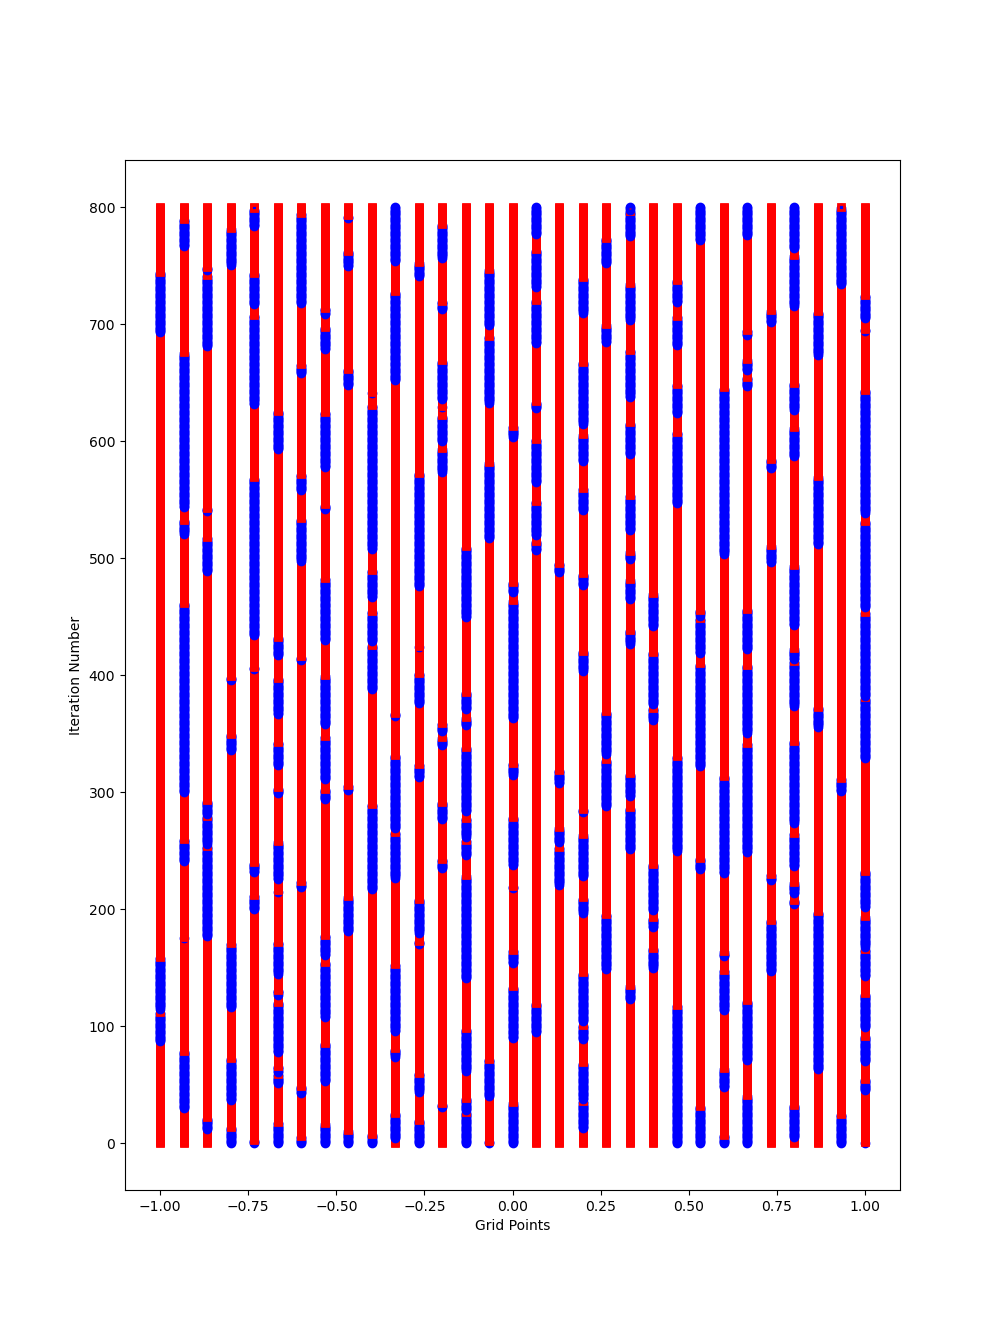
\includegraphics[scale=0.5]{figures/grid-opt/poisson_unitary_grid_time_conv_only.png}
  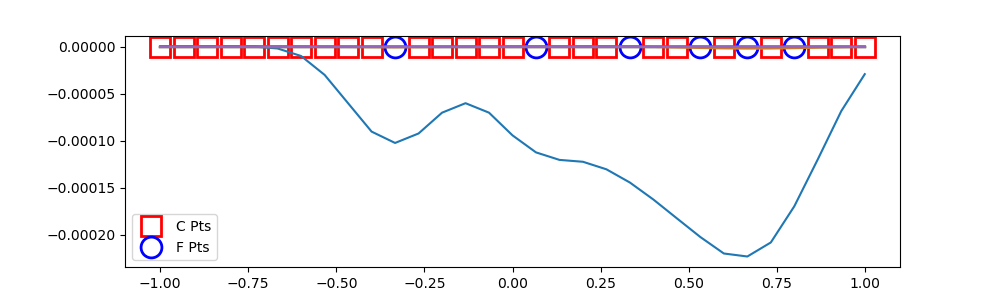
\includegraphics[scale=0.5]{figures/grid-opt/poisson_unitary_grid_conv_conv_only.png}
  \caption{(Top) Time evolution of grid obtained by optimizing CNN output on a normal poisson problem, initial grid on bottom and final grid on top.  (Bottom) convergence behaviour of the resulting grid.  This was computed using simulated annealing, though only optimizing on the \textit{convergence factor}.  True convergence factor: $0.14123$, predicted factor: $0.12423$.  C/F ratio: $0.80645$.  Elapsed time: $1.42712$ seconds.  }
  \label{fig:optimized_grid_poisson_conv}
\end{figure}

\begin{figure}[h]
  \centering
  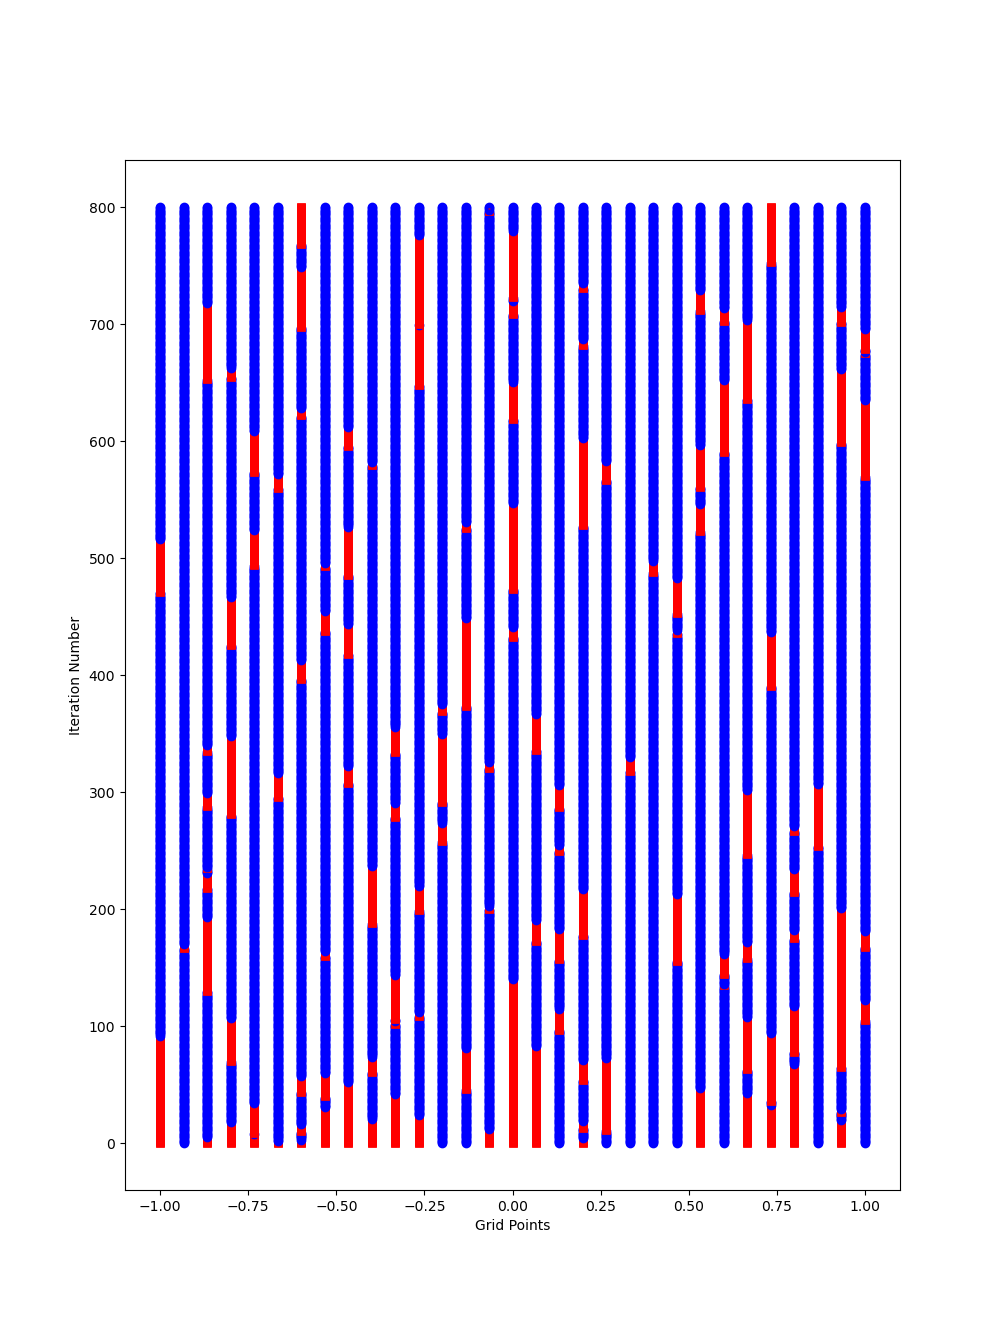
\includegraphics[scale=0.5]{figures/grid-opt/poisson_unitary_grid_time_cf_only.png}
  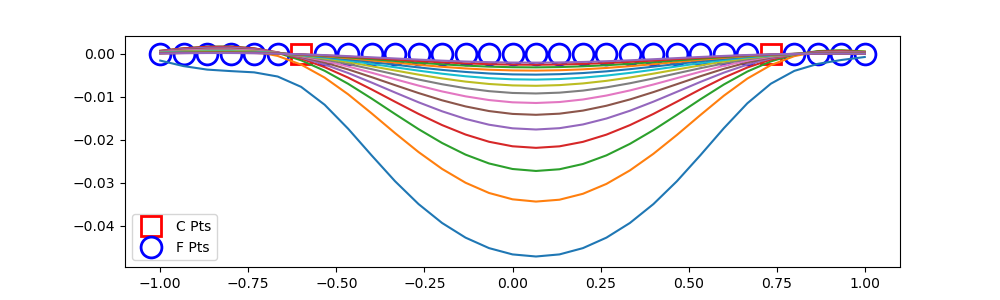
\includegraphics[scale=0.5]{figures/grid-opt/poisson_unitary_grid_conv_cf_only.png}
  \caption{(Top) Time evolution of grid obtained by optimizing CNN output on a normal poisson problem, initial grid on bottom and final grid on top.  (Bottom) convergence behaviour of the resulting grid.  This was computed using simulated annealing, though only optimizing on the \textit{C/F ratio}.  True convergence factor: $0.92223$, predicted factor: $0.91534$.  C/F ratio: $0.064516$.  Elapsed time: $0.91058$ seconds.  }
  \label{fig:optimized_grid_poisson_cf}
\end{figure}

\begin{figure}[h]
  \centering
  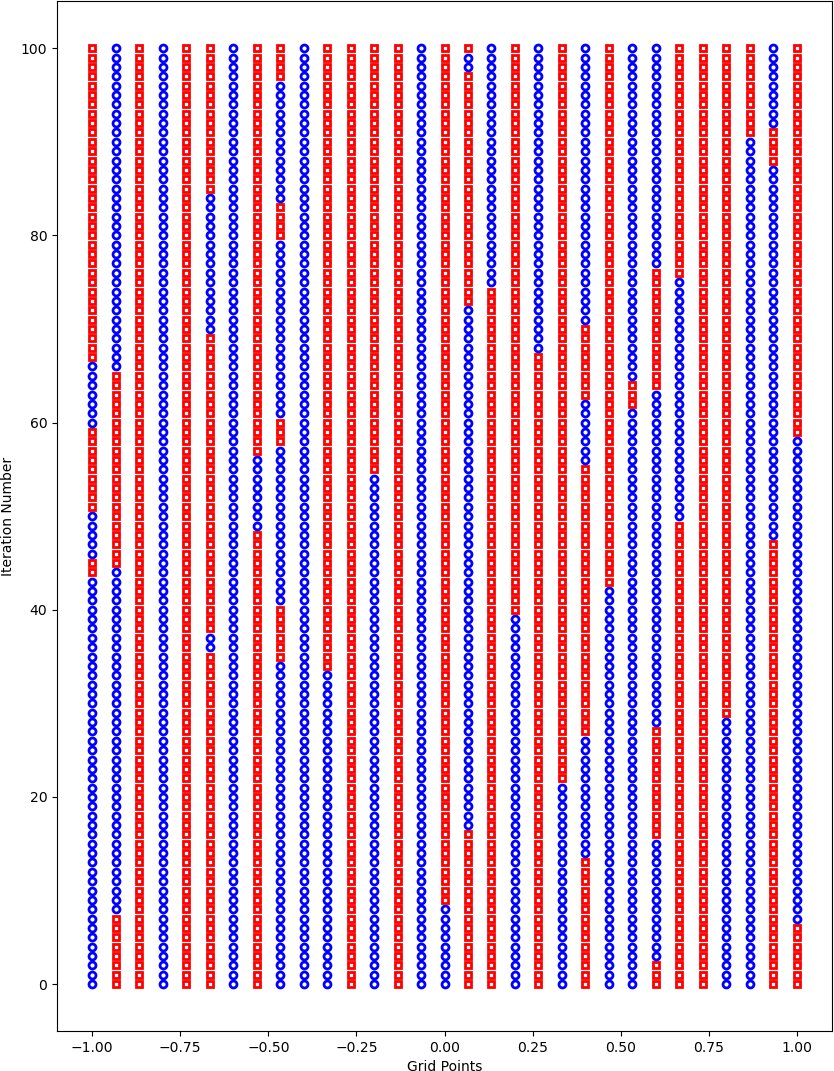
\includegraphics[scale=0.5]{figures/grid-opt/poisson_unitary_grid_time.png}
  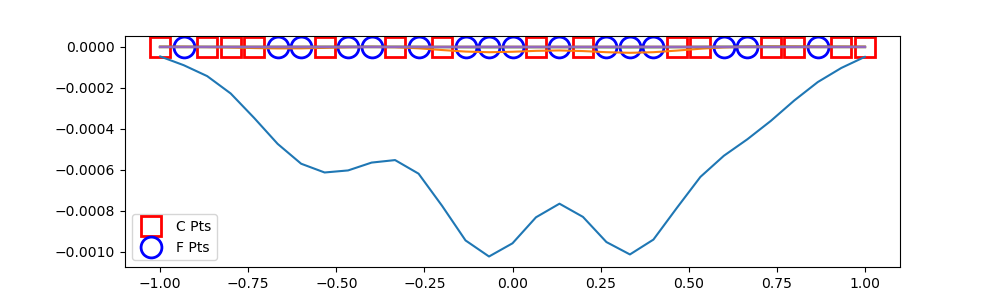
\includegraphics[scale=0.5]{figures/grid-opt/poisson_unitary_grid_conv.png}
  \caption{(Top) Time evolution of grid obtained by optimizing CNN output and C/F ratio on a normal poisson problem, initial grid on bottom and final grid on top.  (Bottom) convergence behaviour of the resulting grid.  This was computed using simulated annealing as described in Algorithm \ref{anneal}.  True convergence factor: $0.37479$, predicted factor: $0.38923$.  C/F ratio: $0.48387$.  Elapsed time: $1.4640$ seconds.  }
  \label{fig:optimized_grid_poisson}
\end{figure}

\begin{figure}[h]
  \centering
  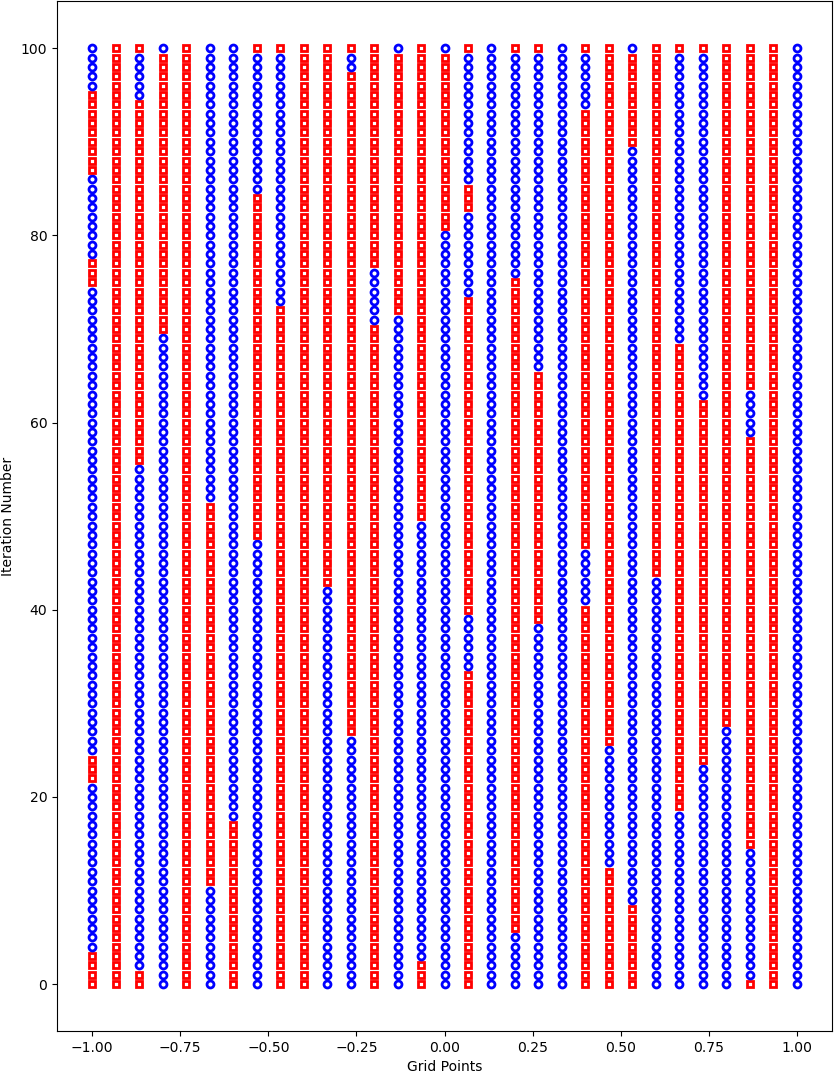
\includegraphics[scale=0.4]{figures/grid-opt/poisson_sine_grid_time.png}\\
  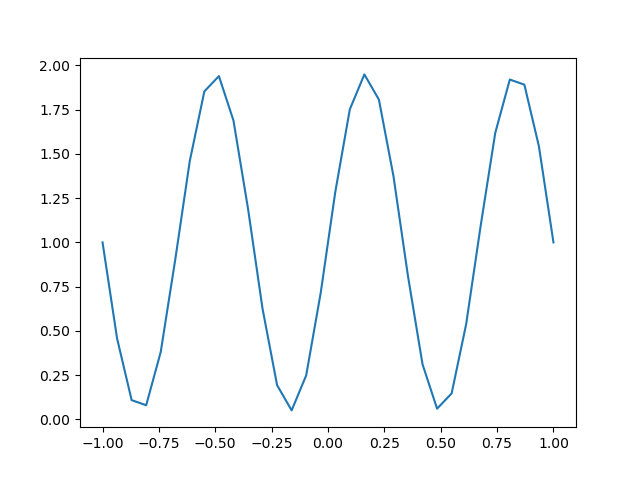
\includegraphics[scale=0.3]{figures/grid-opt/poisson_sine_coeffs.png}
  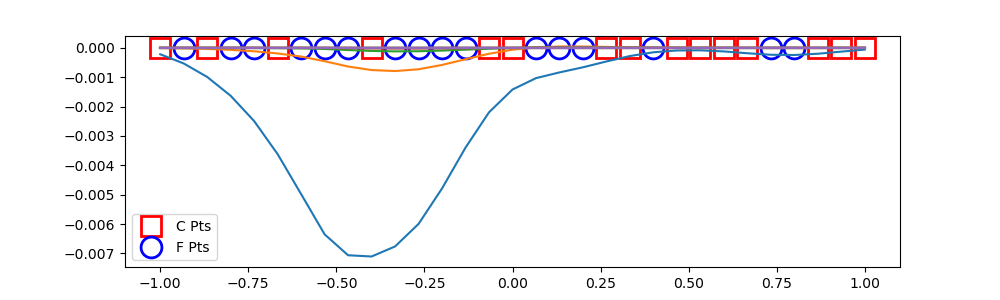
\includegraphics[scale=0.3]{figures/grid-opt/poisson_sine_grid_conv.png}
  \caption{(Top) Time evolution of grid obtained by optimizing CNN output on the variable coefficient poisson problem, initial grid on bottom and final grid on top.  (Left) Variable coefficient function, $k(x)=1+0.95\sin\left(\pi x\right)$.  (Right) final convergence behaviour.  True convergence factor: $0.47893$, predicted factor: $0.85469$.  Elapsed time: $1.47459$ seconds.  }
  \label{fig:optimized_grid_varcoeff}
\end{figure}

%% \begin{figure}[h]
%%   \centering
%%   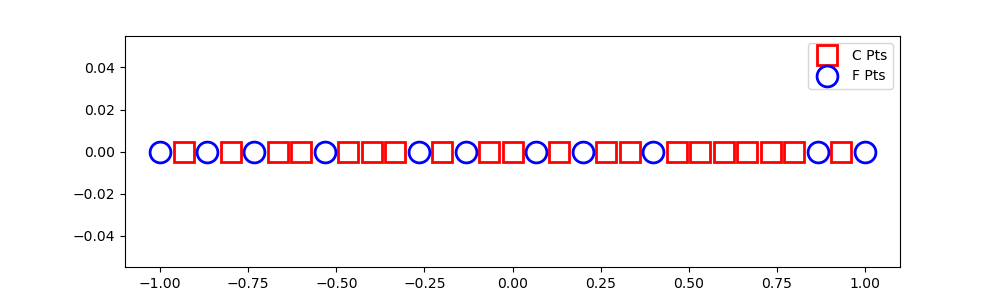
\includegraphics[scale=0.7]{figures/jacobi-conv/conv_opt_grid.png}
%%   \caption{Grid obtained by optimizing CNN output.  This was computed using SciPy's Basin-hopping optimizer.  True convergence factor: $0.1464$, predicted factor: $0.1571$.}
%%   \label{fig:optimized_grid}
%% \end{figure}

%% \begin{figure}[h]
%%   \centering
%%   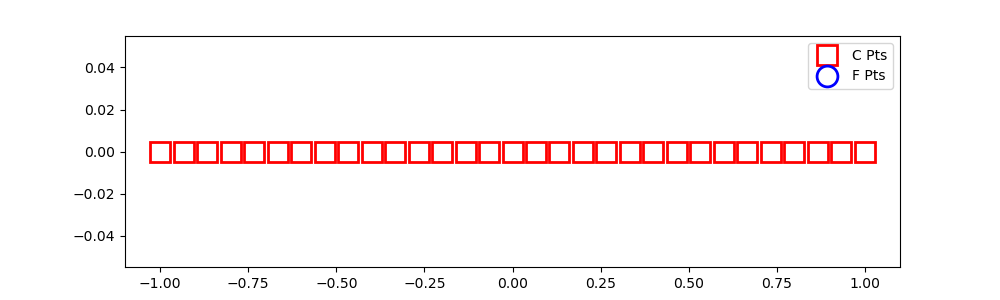
\includegraphics[scale=0.7]{figures/jacobi-conv/conv_opt_grid_in_data.png}
%%   \caption{Grid in the testing/training data that minimizes convergence factor.  This is just a grid of all coarse points, which reduces to a direct solve.}
%%   \label{fig:optimized_grid_in_data}
%% \end{figure}

\nocite{*}
\bibliographystyle{siam}
\bibliography{jacobi-conv-cnn}

\end{document}
